\documentclass[11pt,a4paper]{scrbook}

%---------- Packages ----------
\usepackage[latin1]{inputenc}
\usepackage{xspace}
\usepackage{hyperref}
\usepackage{booktabs}
\usepackage{listings}
\usepackage{graphicx}
\usepackage{subfig}
\usepackage{tikz}
\usepackage{geometry}
\usepackage{fancyhdr}

\newcommand{\libalf}{\texttt{libALF}\xspace}
\newcommand{\cpp}{C+$\!$+\xspace}
\newcommand{\java}{\texttt{Java}\xspace}
\newcommand{\offline}{\emph{offline}\xspace}
\newcommand{\online}{\emph{online}\xspace}
\newcommand{\teacher}{\emph{teacher}\xspace}
\newcommand{\alphsize}{\emph{alphabet size}\xspace}
\newcommand{\conjecture}{\texttt{conjecture}\xspace}
\newcommand{\cj}{\texttt{cj}\xspace}
\newcommand{\advanced}{\emph{advance}\xspace}
\newcommand{\memque}{\emph{membership queries}\xspace}
\newcommand{\accepted}{\emph{accepted}\xspace}
\newcommand{\rejected}{\emph{rejected}\xspace}
\newcommand{\result}{\texttt{result}\xspace}
\newcommand{\stringtype}{\texttt{String}\xspace}
\newcommand{\inputs}{\texttt{input}\xspace}
\newcommand{\checkeq}{\texttt{check\_equivalence\(\)}\xspace}
\newcommand{\answer}{\texttt{answerMembership}\xspace}
\newcommand{\getqueries}{\texttt{get\_queries\(\)}\xspace}
\newcommand{\getsize}{\texttt{get\_alphabetsize\(\)}\xspace}
\newcommand{\filters}{\emph{filters}\xspace}
\newcommand{\normalizers}{\emph{normalizers}\xspace}
\newcommand{\vectored}{\texttt{vector}\xspace}
\newcommand{\node}{\texttt{node}\xspace}
\newcommand{\integer}{\texttt{integer}\xspace}
\newcommand{\true}{\texttt{true}\xspace}
\newcommand{\false}{\texttt{false}\xspace}


%---------- Make index ----------
\makeindex

%---------- Title & Author ----------
\title{The \texttt{libalf} Library}

%---------- Document begins ----------
\begin{document}

%---------- fancy headings ----------
\pagestyle{fancy}


%---------- Title ----------
\maketitle{}


%---------- Table of Contents ----------
\tableofcontents
\listoffigures
\cleardoublepage

%---------- Content ----------

\chapter{Introduction}

\section{LibALF Basics}
		The \libalf library is an actively developed, stable, and extensively-tested library for learning finite state machines. It unifies different kinds of learning techniques into a single flexible, easy-to-extend, open source library with a clear and easy-to-understand user interface.
		\paragraph{}	
		The \libalf Library provides a wide range of \online and \offline algorithms for learning Deterministic (DFA) and Non Determinisitc Finite Automaton (NFA). \online algorithm is a technique where the hypothesis is built by understanding the classification (whether accepted or rejected) of queries asked to some kind of a \teacher.  While, an \offline algorithm builds an apposite hypothesis from a set of classified examples that were passively provided to it. As of \today, the library contains seven such algorithms implemented in it which are listed in Table \ref{algtables}.

		\begin{table}
		\centering
		\begin{tabular}[c]{lcr}
		\toprule[1pt]
			Online Algorithms & Offline Algorithms \\	
		\midrule
			Angluin's L [2] (two variants) & Biermann [3] \\
			NL [4] & RPNI [13] \\
			Kearns / Vazirani [10] & DeLeTe2 [6]\\
		\bottomrule[1pt]
		\end{tabular}
		\caption{List of Algorithms Implemented}
		\label{algtables}
		\end{table}
		
	  \paragraph{}	
		The central aim of \libalf Library is to provide significant advantages through potential features to the user. Our design of the tool primarily focuses on offering high flexibility and extensibility. 
	  \paragraph{}	
		Flexibility is realized through two essential features the library offers. The first being the support for switching easily between learning algorithms and information sources, which allows the user to experiment with different learning techniques. The second being the versatility of the tool. Since it is available in both \cpp and \java (using the Java Native Interface), it can be used in all familiar operating systems (Windows, Linux and MacOS in 32- and 64-bit). In addition, the dispatcher implements a network based client-server architecture, which allows one to run \libalf not only in local environment but also remotely, e.g., on a high performance machine.
		\paragraph{}
		In contrast, the goal of extensibility is to provide easy means to augment the library. This is mainly achieved by \libalf's easy-to-extend design and distributing \libalf freely as open source code. Its modular design and its implementation in \cpp makes it the ideal platform for adding and engineering further, other efficient learning algorithms for new target models (e.g., B?chi automata, timed automata, or probabilistic automata). 
		\paragraph{}
		Other pivotal features of the library include, ability to change the \alphsize during the learning process, extensive logging facilities, domain-based optimizations via so-called normalizers and filters, GraphViz visualization.
		
		
\section{Conceptual Details}

	The \libalf consists of four main components, the Learning Algorithm, the Knowledgebase, Filters \& Normalizers and Logger \& Statistics. Figure \ref{fig:components} shows a characteristic view of the these components. Our implemention of these components allows for plug and play usage.

\begin{figure}[h]
  \centering
  \subfloat[Algorithms]{\label{fig:alg}\includegraphics[width=0.35\textwidth,scale=0.3]{Images/1.png}}  \hspace{30pt}           
  \subfloat[Knowledgebase]{\label{fig:base}\includegraphics[width=0.3\textwidth]{Images/2.png}}\\
  \subfloat[Filter \& Normalizer]{\label{fig:filter}\includegraphics[width=0.27\textwidth]{Images/3.png}} \hspace{30pt}
  \subfloat[Logger \& Statistics]{\label{fig:logger}\includegraphics[width=0.35\textwidth]{Images/4.png}}
  \caption{Components of LibALF}
  \label{fig:components}
\end{figure} 
	
\subsection{The Knowledgebase}

	The knowledgebase is an efficient storage for language information that accumulates every word and its associated classification. It allows storage of values of arbitrary types and in the forthcoming sections we will describe its implementation where a word is stored as a list or array of \texttt{Integers}.
	It forms the fundamental source of information for a learning algorithm. Using an external storage for the knowledgebase has the advantage of it being independent of the choice of the learning algorithm. This enables interchanging of learning algorithms on the basis of same knowledge available. 
	
\begin{figure}[h]
	\centering
	\subfloat{\label{fig:baseandalg}\includegraphics[width=0.5\textwidth]{Images/combined3.png}}
	\subfloat{\label{fig:basealgfilt}\includegraphics[width=0.5\textwidth]{Images/combined5.png}}
	\caption{Pictorial Representation of Plug and Play support}
	\label{fig:plug}
\end{figure}

\subsection{Learning Algorithm}
	A learning algorithm is a component that retrieves the desired information from the knowledgebase to construct a conjecture. As mentioned in the previous section, there exists two types of learning algorithms - \offline and \online algorithm. 
	\paragraph{}
	The workflow of the algorithms begins with a common step wherein the algorithm is supplied with information about size of the alphabet for the conjecture. Thereafter, the algorithms follow two separate procedures to compute the conjecture.
	
	The \offline algorithm continues as stated below.
\begin{enumerate}
	\item The knowledgebase is furnished with the set of words and their classifications (provided by the user).
	\item When all details have been supplied and is available in the knowledgebase, the learning algorithm is made to advance to 	compute the conjecture in conformance with the samples.
\end{enumerate}

	An \online algorithm proceeds in the following manner. \\
	The following two steps are repeated until a correct conjecture is determined.
\begin{enumerate}
\item The algorithm is made to advance.
\item Here one of the following two possibile events may occur.
\begin{enumerate}
\item If no hypothesis is created, ``membership queries'' that require associated classification are resolved (by the \teacher) and added to the knowledgebase.
\item If a hypothesis was created, the ``equivalence query'' is answered by the teacher. If the conjecture is incorrect a counter example is rendered by the teacher.
\end{enumerate}
\end{enumerate}	
	
An insight into the working of the two algorithms is given in Section 1.3.
	
\subsection{Filters and Normalizers}	
	The knowledgebase can be associated with a number of \filters, which are used for domain-specific optimization. This implies that the knowledgebase makes use of domain-specific information to reduce the number of queries to the teacher. Such filters can be composed by logical connectors (and, or, not). In contrast, \normalizers are able to recognize words equivalent in a domain-specific sense to reduce the amount of knowledge that has to be stored. 
		
\subsection{Loggers and Statistics}	
	The library additionaly features means for statistical evaluation or loggers. A logger is an adjustable logging facility that an algorithm can write to, to ease application debugging and development. The modularity of our approach in developing \libalf facilitates these components to be added in an easy plug and play fashion and that is shown in Figure \ref{fig:plug} and Figure \ref{fig:loggers}.
	
\begin{figure}[h]
	\centering
	\includegraphics[width=0.5\textwidth]{Images/combined6.png}
	\caption{Addition of Loggers and Statistics in Plug and Play fashion}
	\label{fig:loggers}
\end{figure}
	
\subsection{Connections of the Components}

The primary aspect in describing the working would be to outline the data flow between a learning algorithm, the knowledgebase and the user (or \emph{teacher}) as sketched in Figure \ref{communications}.

\begin{figure}
\centering
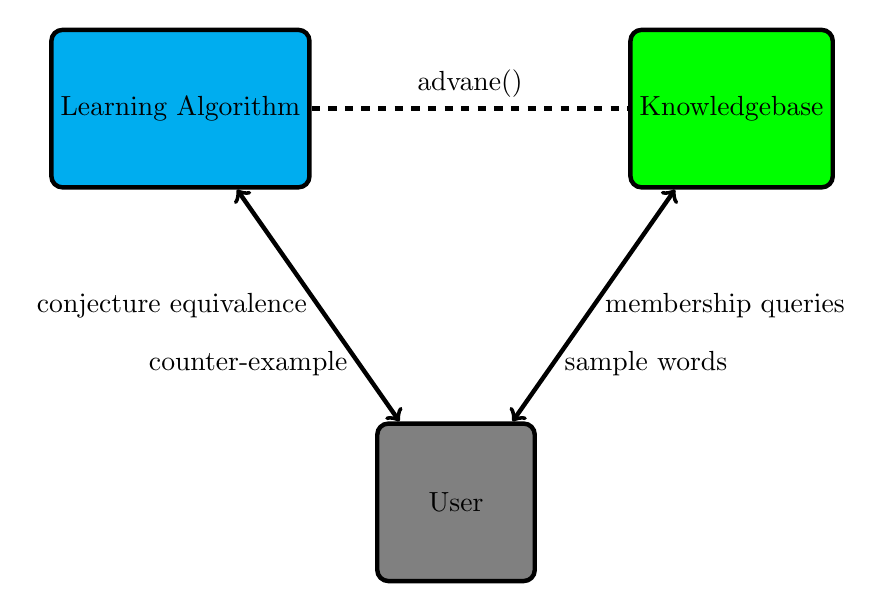
\begin{tikzpicture}[rounded corners,ultra thick]
\draw node[minimum height=2cm,minimum width=2cm,fill=cyan,draw] (la) at (0,5) {Learning Algorithm};
\draw node[minimum height=2cm,minimum width=2cm,fill=green,draw] (kn) at (7,5) {Knowledgebase};
\draw node[minimum height=2cm,minimum width=2cm,fill=gray,draw] (user) at (3.5,0) {User};
\draw[dashed,ultra thick] (la) -- (kn) node[midway,above] {advane()};
\draw[<->,ultra thick] (la) -- (user) node[midway,left] {conjecture equivalence} node[near end,left] {counter-example};
\draw[<->,ultra thick] (kn) -- (user) node[midway,right] {membership queries} node[near end,right] {sample words};
\end{tikzpicture}
\caption{data flow of the \libalf components}
\label{communications}
\end{figure}

The learning algorithm and the knowledgebase share information with user. The knowledgebase, as stated earlier, is the fundamental information for the learning algorithm to develop an automaton. The learning algorithm advances with whatever knowledge is available. The learning algorithm connects with the user to collect relevant information such as equivalence of a conjecture or to retrive counter-example. When the learning algorithm creates more membership queries, they are stored in the knowledgebase leading to it initiating a communication with the user who is required to answer membership queries (or input sample words in case of an offline algorithm). All such information extended by the user are stored in the knowledgebase. 

\section{Demo Application}

In this section we describe the working of the \offline and \online algorithms with reference to the demo code in \cpp available at our website \url{http://libalf.informatik.rwth-aachen.de/}. Demo programs of the algorithms in \java are also available there.

The following code snippet briefly demonstrates how to employ the \libalf library in a user application. It is important that you become familiar with the auxilliary methods used in the program and hence their operations are explained first.

\begin{itemize}
\item \textbf{\emph{get\_AlphabetSize()}} - Promts the user to provide information about the size of alphabet and stores it as an \texttt{Integer}.
\item \textbf{\emph{answer\_Membership(\*li)}} - Takes the list of queries as an arguement and presents it to the user to classify them. It returns \texttt{true} when the word is to be accepted and returns \texttt{false} when it is to be rejected.
\item \textbf{\emph{check\_Equivalence(cj)}} - Presents the computed conjecture to the user who marks it as correct or incorrect. Returns \texttt{true} or \texttt{false} respectively.
\item \textbf{\emph{get\_CounterExample(alphabetsize)}} - Requests the user to input the counter-example and returns the word as a list (array in \java implementation) of integers. It takes the alphabetsize as a parameter for validation purposes.
\item \textbf{\emph{get\_Samples(alphabetsize)}} - Retrieves the sample word from the user. The alphabetsize is passed as a parameter for validation purposes.
\item \textbf{\emph{classification = get\_Classification()}} - Retrieves the classification of the sample word from the user. Returns \texttt{true} when the word is to be accepted and returns \texttt{false} when it is to be rejected.
\item \textbf{\emph{enough\_Samples()}} - Requests the user to specify whether all samples have been provided by the user. Returns ``y'' if user desires addition of more samples or ``n'' if all samples have been provided already.
\end{itemize}

\subsection{Online Algorithm}

An \online Algorithm, as mentioned in the previous section, formulates the conjecture by putting forth ``queries'' to the \teacher.

\lstset{language=c++, numbers=left, numberstyle=\tiny, stepnumber=1, numbersep=5pt}
\begin{lstlisting}[frame=single]
void main(int argc, char**argv) {
int alphabetsize = get_AlphabetSize();
knowledgebase<bool> base;
angluin_simple_table<bool> algorithm(&base,
NULL,alphabetsize);
do {
 conjecture * cj = algorithm.advance();
 if (cj == NULL) 
 {
   list<list<int> > queries = base.get_queries();
   list<list<int> >::iterator li;
   for(li = queries.begin(); li != queries.end(); li++) 
   {
      bool a = answer_Membership(*li);
      base.add_knowledge(*li, a);
   }
 }
 else 
 {
   bool is_equivalent = check_Equivalence(cj);
   if (is_equivalent) result = cj; 
   else 
   {	
      list<int> ce = get_CounterExample(alphabetsize);
      algorithm.add_counterexample(ce);
   }
 }
}while (result == NULL);
cout<<result->visualize();
}
\end{lstlisting}

The workflow of the program is as described below:

\begin{enumerate}
	\item At line 2, the program promts the user to input the \alphsize of the Automaton.
	\item An empty knowledgebase is now intialized at line 3. (The knowledgebase stores the words as a list of \texttt{Integers})
	\item Now, a learning algorithm is created by providing three parameters - the knowledgebase, NULL for a logger, the Alphabet Size.
	\item After having initialized the learning algorithm, the program is subjected to a loop where the algorithm is made to \advanced (Line 7). The result of this is stored in a \conjecture type variable \cj.
	
	\item If there was no sufficient information available in the knowledgebase to construct a conjecture, then \cj is NULL and the algorithm enters the condition at line 8. The algorithm produces the \memque that needs to be resolved by the user (or \teacher). The queries are obtained using the method \getqueries. (Note: the queries are obtained in ``list of list of \texttt{Integers}'' since words are stored as \texttt{Integers} and there may be more than one query)
	
	\item The queries produced are presented to the user who classifies it as \accepted or \rejected. This is done at Line 13 with \answer function. Subsequently, This information is added to the knowledgebase and the iteration of the loop continues.

	\item However, if a conjecture was computed at line 7, (implying that enough information was available in the knowledgebase), then algorithm enters the condition at line 18. The conjecture is presented to the user by \checkeq function at line 20.
	
	\item If the conjecture is equivalent, the user marks it correct and the conjecture is stored in variable \result. Iteration ends and the \result is displayed in line 32.
	
	\item If it is not equivalent, the user is now prompted to provide a counter example (line 27) and the program continues with the iteration. Typically, the counter example would influence the learning algorithm to invoke more \memque that is to be resolved during the next \advanced of the algorithm.
\end{enumerate}

\subsection{Offine Algorithm}

An \offline algorithm, as mentioned in the previous section, computes a conjecture from a set of passively provided input samples with their classifications.

\lstset{language=c++, numbers=left, numberstyle=\tiny, stepnumber=1, numbersep=5pt}
\begin{lstlisting}[frame=single]
int main(int argc, char**argv) 
{
  int alphabetsize = get_AlphabetSize();
  string input = "y";
  list<int> words;
  bool classification;
  knowledgebase<bool> base; 
  while (input == "y") 
  {
    words = get_Samples(alphabetsize);
    classification = get_Classification();
    base.add_knowledge(words, classification);
    input = enough_Samples();
  }
  RPNI<bool> algorithm(&base, NULL, alphabetsize);
  conjecture *cj = algorithm.advance();
  cout <<cj->visualize();
}
\end{lstlisting}

The workflow of the above program is as follows:

\begin{enumerate}

\item At line 2, the program prompts the user to input the \alphsize used for the automaton (coded in the function \getsize)
\item Variables for storing the sample words and their classifications are described subsequently. An empty knowledgebase is now initialized. 
\item The program then passes over a loop which recursively performs the action of reading the sample (line 10) and its classification (line 11) from the user. As and when the user inputs this information, it is continually added to the knowledgebase (line 13). The loop ends when the user indicates that the desired number of samples have been entered as coded in line 13 (its for this purpose that the \stringtype \inputs is first initialized to ``y'').
\item Now, a learning algorithm (RPNI Offline Algorithm) is created by providing three parameters - the knowledgebase, NULL for a logger, the Alphabet Size (line 15)
\item Having initialized the algorithm, it is now made to \advanced which produces a conjecture that pertains to the user's specification of samples. (line 16)
\item Finally, the conjecture is printed as coded in line 17 of the program.

\end{enumerate}

In both the command line programs implemented in \cpp and \java, the program outputs the ``.dot'' file which contains the code that builds the conjecture graphically. (This file may be executed using the GraphVIZ tool).




\chapter{Installation}
The \libalf library contains all functionality to embed different kinds of (offline and/or online algorithms) into your learning application. It can be used as C++ library directly, via JNI (Java Native Interface) or via a dedicated client/server application called the dispatcher. Both may be used from Java interchangable via the generic interface ``jalf''.
The chapter gives information on how to install \libalf in a user application under Windows and Linux operated systems.

\section{Requirements}
In general, \libalf is platform independent. It has been tested in both x86 and x64 systems successfully. To use \libalf, your computer must have the following softwares installed.
\begin{enumerate}
 \item \textbf{GNU Compiler} \vskip 1pt
	For windows, we recommend usage of MinGW compiler for using \libalf. Instructions on where to find it and how to install it are given in section --.
 \item \textbf{Java 1.x} \vskip 1pt
	This is required to use \libalf via JNI. \libalf can be compiled using \texttt{ant}.
\end{enumerate}
\paragraph{Note:}
The dispatcher can be compiled only under linux since it uses POSIX which is not compatible under windows. 

\section{Installing MinGW compiler in Windows}
We recommend the usage of MinGW compiler for users who would like to use \libalf in Windows. Instructions on how to install it is given below.
\subsection*{Where to find it and how to install it}
The downloadable package and installation instructions of the MinGW compiler can be found in the following website.

\url{http://www.mingw.org/wiki/HOWTO_Install_the_MinGW_GCC_Compiler_Suite}

\textbf{Note:} Installing MinGW compiler on your computer does not automatically set the ``PATH'' variable. You may have to manually update the “PATH” variable of the computer to the ``bin'' folder of MingW. (Usually ``C:\textbackslash MingW\textbackslash bin'', unless you have changed the directory of installation). 
of \libalf.
\paragraph{How to edit the environment variables}
\begin{enumerate}
 \item Right click \textbf{My Computer}, Click ``Properties''.
 \item Click the ``Advanced'' tab and click ``Environment Variables''.
 \item Under the frame ``system variables'', find and click on the variable named \textbf{path} and click edit.
 \item In the textbox beside ``Variable value'', add ``c:\textbackslash MinGW\textbackslash bin'' (or the location of the ``bin'' folder where you have installed the compiler) by separating it with a semicolon (;) from the existing path. Please make sure that you do not delete the existing paths set in the variable.
 \item  Click Ok. And click Ok in the window displaying the ``system variables''.
\end{enumerate}
As soon as the MinGW compiler is installed, please follow the steps listed below to be able to compile \libalf.

\subsection*{Modification to the MinGW compiler}

As a prerequisite towards compiling the Library a small change is made to the “bin” folder of the MingW.   
After the installation of the MingW compiler, the ``/bin'' folder will contain an executable file named \textbf{mingw32-make.exe}. It is required that this file is renamed to \textbf{make.exe} since the commands in the makefiles are written as \textbf{make \emph{sourcefilename}} and not as \textbf{mingw32-make \emph{sourcefilename}}.

\section{The \libalf \cpp Library}
The section describes how to compile the sources and use the \cpp library directly in your application.
\subsection*{Compiling \libalf}
A ``makefile'' is provided already to compile \libalf. \vskip 1pt
To compile the library in linux, use the following command.
\[
  PREFIX = <path> make
\]
\emph{$<$path$>$} must specifiy the directory where the \libalf sources are located. This is because \texttt{make} searches the \emph{include} directory inside the directory specified by PREFIX for the \libalf's header files. If you do not wish to use gcc compiler or if gcc is not installed in /usr/bin/gcc, you can additionally specify the CC variable pointing to your desired \cpp compiler. \vskip 1pt
To compile the library in Windows, go to \textbf{Command Prompt} and enter the following command.
\[
 make -f <path>/makefile
\]
\subsection*{Employing \libalf in an Application}
To use the installed library in your application, follow the steps given below. \vskip 1pt
On windows, one of the following methods can be used
\begin{enumerate}
 \item Place the compiled library into the directory where your application is located.
 \item Alternatively, you can add the path containing the \libalf library in to your \textbf{path} variable.
\end{enumerate}
On Linux, you use the LD\_LIBRARY\_PATH to point to \libalf's location.
\[
  LD\_LIBRARY\_PATH = <path>/bin
\]

\section{The \libalf Java Library}
The section describes how to install the Java sources of \libalf and use them in your application.
\subsection*{Compiling \libalf}
To compile the Java based \libalf library, you may use ANT (\url{http://ant.apache.org/}). \vskip 1pt
In both Windows and Linux, the following command can be used.
\[
  ant -D PREFIX=<path>
\]
Here, the variable \emph{path} specifies the directory where the ``jalf.jar'' is located. The option -D is used to specify variables (in this case it adds the ``jalf.jar'' to Java's classpath). \vskip 1pt

\subsection*{Employing \libalf in an Application}
To use \libalf in your application, you must make sure that the compiled jalf library and the ``jalf.jar'' can be found. \vskip 1pt
In both Windows and Linux, you can do this by specifying the following two parameters.
\begin{enumerate}
 \item -classpath ``$<$path$>$:.'' \vskip 1pt
	Use the command to set the classpath to point to ``jalf.jar''. \vskip 1pt
	\textbf{Note:} The seperator ``:'' must be used on Linux and ``;'' must be used on Windows.
 \item -D java.library.path = $<$path$>$ \vskip 1pt
	Use the command to let the java library path variable point to the compiled jalf library. 
\end{enumerate}

\section{Troubleshooting}
If you have problems compiling the library using \texttt{make} in windows, it could be because of Linux commands used in the makefiles. Ordinarily, MinGW should not have problems compiling it. But if problems do exist, then download and install \textbf{makeutils} which can be found at \url{http://makeutil.sourceforge.net/#download}. \vskip 1pt
Please make sure that the ``/bin'' folder of makeutil is added to your \texttt{path} variable. If the installation does not do it automatically, do it manually in the same way as described in -- under ``\textbf{How to edit environment variables}''.

\section{Dependencies}
\libalf is a stand-alone C++ library and does not depend on any other libraries except the C++ standard library and standard template library (STL). Also, MiniSat v1.14 is fully integrated into libalf, as it is required for the bierman learning algorithm. There are no further dependencies.

However, the following libraries may be of help when developing applications and are partially required for some of the testcases:

\begin{enumerate}
 \item \textbf{libAMoRE-1.0 / libAMoRE++} : C/C++ automata library for working with finite automata. 
(Both AMoRE-1.0 with some patches and the C++ interface currently reside in the subversion repository of libalf. the C++ interface has  been written during development of libalf, but we're currently working on integrating it into the original libAMoRE (upstream).)
 \item \textbf{liblangen} (LANguageGENerator) is a library for generating (regular) languages in the form of automata or regular expressions. It came to existence during the development of libalf and thus has the same interface for automata. it is useful e.g. for generating random automata or regex with specific constraints, so algorithms can automatically massively be tested.
\end{enumerate}

\section{License Information}
\libalf is a free software published under the LGPL v3 license.Under this license, you have the complete freedom for the following.
\begin{enumerate}
 \item Use the software for any purpose.
 \item Make copies and redistribute the software.
\end{enumerate}
You also gain the complete freedom to modify the software according to your needs and distribute the modified version of the software. However, the modified software must be published with the code under the LGPL v3 (any later version) license. 
For more information about LGPL license, visit \url{http://www.gnu.org/licenses/lgpl.html}




\chapter{The Knowledgebase}

The knowledgebase is the central repository of information. It is a database that stores words and their classification. Apart from this basic functionality, the knowledgebase also offers number of other features thereby increasing extensibility support. 
But we have not designed our knowledgebase to do just that but also to provide extensibility. In this regard, the methods used implementation of knowledgebase can be divided into two categories - \textbf{\emph{Methods important for Using \libalf}} and \textbf{\emph{Methods important for expanding \libalf}}. 
\paragraph{}
In this chapter, we shall discuss the knowledgebase from a user's perspective and a developer's perspective. The material will include adequate account of its structure, operations and implementation.  The final section of this chapter will provide an appendix of all the methods used in programming the knowledgebase with a brief description corresponding to it.  

(A PICTURE OF KNOWLEDGEBASE FROM DEMO HERE)

\section{The knowledgebase - A User's Perspective}

\paragraph{} In this section, we describe the basic functionality of the knowledgebase. The following material provides fundamental information that one would have to know to employ \libalf in an application. This section will not deal with explanation of the internal structure or methods used for operations of the knowledgebase. However, it will provide some elementary details of methods that could be required to better understand an operation.  To discover more on those areas, you may refer the section on Developer's Perspective and Methods in Detail.

\subsection*{Basic Concepts}
	
	To understand the functions of the knowledgebase, it is important to know the basic underlying concepts. We shall define some key terms for a start.
	
\paragraph{Symbol} It is an arbitrary data which has some meaning to or effect on the machine. It is elementary data on which an automaton is built. 

\paragraph{Alphabet} It is a finite set of symbols. An alphabet set is usually denoted by $\Sigma$.
\vskip 1pt
\[
\sum = \{0,1,\ldots\}
\]

For example, in \libalf, when alphabet size of two is specified by the user, then by default the alphabets involved in the automaton would be 
\[
\sum = \{0,1\}
\]

This leads us to define the following.

\paragraph{Word} A finite string formed by the concatenation of a number of symbols.

\paragraph{Language} Language is a set of words, formed by symbols in a given alphabet.

Thus, adding to our previous example, ``01101'' would be a word from the given set of alphabet and the set \{ 01101, 11011\} would be a Language.

\subsection*{Storing Words} 
The knowledgebase of \libalf is an efficient storage of words and their classifications. Classifications are nothing but the acceptance rules of the word i.e., whether the word has to be accepted or rejected by the automaton. The knowledgebase maintains information about this with the variable \texttt{status}. Since the knowledgebase can use arbitrary values, one may choose to store this information in any form. 

\subsection*{Queries and Answers} 
The next major function of the knowledgebase would be to store queries to help the learning algorithm build the automaton. As mentioned in the previous chapter, a query is nothing but a word whose classification is unknown and needs to be retrieved from the user or teacher. This is called the answer. Hence, given a set of words and classifications, the knowledgebase can store them and when a learning algorithm processes these words, queries created that are also stored in the knowledgebase (which are later presented to the user).

\subsection*{Other features} 
Apart from the essential functions, the knowledgebase also provides certain features that can be made us of when employing it in an application. The knowledge available in the knowledgebase can be also be serialized into the user's hard disk. Also, the knolwedgebase allows one to generate a dot file of the knowledge available to have a graphical representation of the same. All the more, the knowledgebase can also be merged with another knowledgebase without introducing any errors. These features are elaborated in forthcoming sections.

\section{Structure of the Knowledgbase - A Developer Perspective}

\subsection{Representation of a word in the Knowledgebase}
\paragraph{}
	Ideally, the first step towards understanding the organization of the knowledgebase would be to realize how a word is represented in it.
\paragraph{}
	Generally, the knowledgebase can be described as a tree structure with nodes representing the words. More precisely, it is a prefix tree. Given this description and the demo programs from the website (which even presents a graphical representation of the tree), one would imagine a word \texttt{01101} in the knowledgebase as a tree with a node that holding a \stringtype or \texttt{list of integers} with value ``01101''. However, this is \textbf{NOT} how knowledgebase is implemented in \libalf.
\paragraph{}
	The node by itself does \emph{not} contain the complete word, but only contains the i\textsuperscript{th} symbol of the word. An example can make things clear. 
\paragraph{}	
	Consider a word \texttt{01101}. When this word is added to the knowledgebase, it is not stored as a single \stringtype at a node of the tree, instead the sequence of the symbols that comprise the word construct the branch of the tree with every node representing exactly one symbol. This implies, to represent this word in the knowledgebase, the root (which is always an empty string represented by Epsilon) creates a child node that represtents ``0''. The next symbole of the word ``1'' is now represented in a node which is the child of the node representing its previous symbol ( or the parent node), ``0''. Thus, one can reach the node representing the word \texttt{01101} by following the 0\textsuperscript{th} child of the root node, then further accessing the first child of this node and so on.
\paragraph{}
	Hence, to retrive a word from the tree, one has to traverse down from the root node to the final child node by accumulating the symbols that every node represents. Alternatively, one can also recover the word by ascending from a node to the root and reversing the word obtained. \libalf uses the latter technique. 
	\vskip 1pt

	(A PICTURE OF THE ABOVE EXPLAINED TREE HERE)	
	
\subsection{Description of the Structure}
	
	The knowledgebase is designed as a template class enabling usage of arbitrary values for storing desired information.
	The knowledgebase class contains the node class which describes the variables that are necessary for the node. This class also contains some of the internal methods which are important for both using and expanding \libalf.
	The constructor of the node class creates the tree, more precisely (a root node) with the following variables that define the node.
	\begin{itemize}
	\item \texttt{parent} \hfill \vskip 1pt A variable of type \node that points to the parent of the node.
	\item \texttt{label} \hfill \vskip 1pt An \integer variable that contains the alphabet that the node represents. (-1 for root node)
	\item \texttt{status} \hfill \vskip 1pt This indicates whether the classification of the word (the word is constructed by traversing through the tree) is required, answered or can be ignored. It is an \texttt{enum} type variable with the respective three values ``NODE\_IGNORE'', ``NODE\_REQUIRED'' and ``NODE\_ANSWERED''. 
	\item \texttt{answer} \hfill \vskip 1pt It is the type of the template class used in the constructing the knowledgbease. 
	\end{itemize}
	
	After constructing the root node, the child nodes are created with the \vectored type \node variable called \texttt{children}. 
	The knowledgebase contains methods that act upon the node for the operations. 
	These variables and methods form the building blocks of knowledgebase. The methods employed in the knowledgebase is described in the next section.

\section{Methods in Detail}

	In this section we will discuss the methods used in the knowledgebase. The description given below pertains more to a developer as it offers greater insight into the workflow of the knowledgebase along with particulars of the methods.
	
\subsection{Nodes}
	
	Having drawn the working of a node, we begin describing some of the functions that concerns the node. These are internal methods and they perform some basic operations as discussed below.
\begin{enumerate}
\item \textbf{node* get\_next(node * current\_child)} \hfill \vskip 1pt
	This function returns the next node or the next child of the current node (which is passed as an arguement). 
	
\item \textbf{node * get\_parent()} \hfill \vskip 1pt
	The method returns the parent of the node under use.

\item \textbf{list$<$int$>$ get\_word()} \hfill \vskip 1pt
	This function returns the word that the current node represents. The method traverses backwards in the tree (ascending from child to parent) and reverses the sequence obtained to build the correct word.
	
\item \textbf{int get\_label()} \hfill \vskip 1pt
	This function returns the label that the node represents.
	
\item \textbf{node * find\_child(int label)} \hfill \vskip 1pt
	The function is used to find the child node with the specified label.
	
\item \textbf{node * find\_descendant(list$<$int$>$ :: iterator infix\_start, list<int>::iterator infix\_limit)} \hfill \vskip 1pt
	This function is used to find the child node specified by a word. It traverses through the tree based on the iteration over the word to find the path that generates the required word.
	
\end{enumerate}

\subsection{Words and Classification}

	In principal, the primary purpose of the knowledgebase is to store the words and classifications that constitutes the base for the learning algorithm to compute an automaton. We discuss the following two functions of the node and a method relating to this important aspect.
\begin{enumerate}
\item \textbf{node * find\_or\_create\_child(int label)} \hfill \vskip 1pt
	This function returns the child node given the label. However, if the node does not exist, it creates the child node with the specified label.
	
\item \textbf{node * find\_or\_create\_descendant(list$<$int$>$::iterator infix\_start, list$<$int$>$::iterator infix\_limit)} \hfill \vskip 1pt
	This function behaves almost similar to the previous one. However, the difference being, it does not operate with a single label but on a word (which is a list of \integer). 
	
\item \textbf{bool add\_knowledge(list$<$int$>$ \& word, answer acceptance)} \hfill \vskip 1pt
	This is the key function that adds information to the knowledgebase. The parameter ``word'' represents the sample word and ``acceptance'' represents the classification of the word. 
	This method simply calls the ``find\_or\_create\_descendant(list$<$int$>$::iterator infix\_start, list$<$int$>$::iterator infix\_limit)'' so that the knowledge will be added only information about the word does not already exist in the knowledgebase.
\end{enumerate}	

\subsection{Queries}

	The next point of discussion would be the part of knowledgebase that handles queries. For instance, an online algorithm produces queries at every ``advance'' of the algorithm. These queries are stored in the knowledgebase and are later presented to the user for classification.
\paragraph{}
	To understand the implementation of query handling in \libalf's knowledgebase, one must first know the functionality of three methods that are crucial for query handling.

\begin{enumerate}
\item \textbf{bool mark\_required()} \hfill \vskip 1pt
	The method returns a boolean value \true if the acceptance or the classification of the node is requried (i.e, ``status'' is NODE\_REQUIRED) or \false if the classification is already known.
	
\item \textbf{bool is\_required()} \hfill \vskip 1pt
	The method returns the ``status'' as \texttt{NODE\_REQUIRED}. It is used to set this status to a particular node under consideration.

\item \textbf{bool is\_answered()} \hfill \vskip 1pt
	The method returns the ``status'' as \texttt{NODE\_ANSWERED}. It is used to set this status to a particular node under consideration.
\end{enumerate}

\vskip 1pt
  The following methods describe the operations associated with queries.

\begin{enumerate}
\item \textbf{knowledgebase * create\_query\_tree()} \hfill vskip 1pt
	The method creates a tree containing the queries to be answered. Therefore, its return type is \texttt{knowledgebase}.
It uses the \texttt{get\_word()} method to retrive the word and uses the \texttt{add\_query()} method add it in the tree.

\item \textbf{int add\_query(list$<$int$>$ \& word, int prefix\_count = 0)} \hfill \vskip 1pt
	The method is primarily used to add the word into the query tree. When the classification of a word has to be known, the method firsst checks if the word already exists with its classification in the knowledgebase (by using the \texttt{find\_or\_create\_child(int label)} method). Hence, if the classification of the word is unknown and does not already exist, the corresponding node will be created and eventually added in the query tree (since this method is used by \texttt{create\_query\_tree(\ldots)}.
  
\item \textbf{list$<$list$<$int$>$$>$ get\_queries()} \hfill \vskip 1pt
	This method returns the list of all the queries present in the knowledgebase (i.e, all words yet to classified). Naturally, the method uses the \texttt{get\_word()} function to build the word.
	
\item \textbf{bool resolve\_query(list$<$int$>$ \& word, answer \& acceptance) and bool resolve\_or\_add\_query(list$<$int$>$ \& word, answer \& acceptance)} \hfill \vskip 1pt
	These two methods can be described together as their functionality is almost similar and differ only in one aspect. Both methods return \true if the classification of the word is already known and \false if it is unknown. While ``resolve\_query()'' only returns \false, ``resolve\_or\_add\_query()'' marks the status of this word as required and then returns \false. Naturally, the former uses ``find\_descendant()'' and the latter makes use of ``find\_or\_create\_descendant()''.

\item \textbf{void clear\_queries()} \hfill \vskip 1pt
	This method is used to remove all the nodes that are identified or marked as a query.
\end{enumerate}
\vskip 1pt
\vskip 1pt
\subsection{Alphabets in Knowledgebase}
	Although we have defined the basic concepts that includes alphabets in this chapter, the knowledgebase does not really store the alphabet size of the automaton specified by the user. The knowledgebase does not construt the tree based on the alphabet size specified by the user and is capable of constructing the tree precisely even if symbols outside the alphabet set are fed in the input (which includes the extra symbols). But, such improper input will lead to the learning algorithm computing a conjecture which might not be the expectation of the user.
	However, the knowledgebase can at any point of time identify and operate on the alphabet size. This can be regarded as the largest symbol that is processed in the knowledgebase. From Section --, we know that for an alphabet size of 2, the largest symbol would be ``1''.
One can use the following two methods available.
\begin{enumerate}
\item \textbf{get largest symbol} \hfill \vskip 1pt
	(Text to be added here)
\item \textbf{check largest symbol} \hfill \vskip 1pt
	(Text to be added here)
\end{enumerate}



Other Important Methods yet to be used in the document

\paragraph{get memory usage}
\paragraph{to string}
\paragraph{print} ?
\paragraph{generate dot file}
\paragraph{merge knowledgebase}
\paragraph{get root ptr}
\paragraph{get node ptr}


Serialize and deserialize

Iterator
begin, qbegin, end, qend

Iterator class!

\textbf{iterator qbegin()}
	This is the method used to get the query node at which the iterator needs to begin. 





\chapter{Learning Algorithms}

A learning algorithm is a component that retrieves the desired information from the knowledgebase to construct a conjecture. 
A conventional way to distinguish learning algorithms is to group them into \online and \offline algorithms. Online learning techniques are capable of actively asking queries to some kind of teacher who is able to classify these queries. Offline algorithms, on the other hand, are passively provided with a set of classified examples from which they have to build the conjecture.

\subsection*{Online Algorithms}

 The online learning process is based on the model of Minimally Adequate Teacher (MAT) wherein the technique invloves two types of queries, namely, \emph{membership queries} and \emph{equivalence queries}. Online learning algorithms build the conjecture by actively asking queries to a \teacher (i.e.\ a user application). \\ The teacher is required to \emph{resolve} the memebership query by providing the classification of the given word. Equivalence queries check whether a derived conjecture is an equivalent description of the target language to be inferred.
\subsection*{Example Code}

\lstset{language=c++, numbers=left, numberstyle=\tiny, stepnumber=1, numbersep=5pt}
\begin{lstlisting}[frame=single]
void main(int argc, char**argv) {
int alphabetsize = get_AlphabetSize();
knowledgebase<bool> base;
angluin_simple_table<bool> algorithm(&base,
NULL,alphabetsize);
do {
 conjecture * cj = algorithm.advance();
 if (cj == NULL) 
 {
    // Get queries from the knowledgebase and 
    // present it to the user to resolve.
 }
 else 
 {
    // Get the conjecture and present it to the user. 
    // If conjecture incorrect, get counter example
 }
}while (result == NULL);
}
\end{lstlisting}


\begin{itemize}
 \item The algorithm runs on iteration which begins at making an \emph{advance} where in the algorithm tries to compute a conjecture with information available in the knowledgebase.
 \item This leads to the rise of membership queries if no conjecture was created. These queries are resolved by the teacher, answer added to the knowledgebase and the algorithm continues the iteration.
 \item On the other hand, if a conjecture was computed, it is presented to the teacher. The algorithm terminates if the conjecture is correct. Otherwise, the iteration continues after the teacher renders a counter example.
\end{itemize}

\subsection*{Offline Algorithms}

Offline algorithms, in contrast to the online variant, is an NP complete problem of finding the smallest DFA consistant with a given set of classified words.
The algorithm is provided with a set S of classified words (called samples) and the algorithm derives a conjecture which conforms to these samples. 

\paragraph{}
The working of this algorithm follows a simple two step procedure. 
\begin{itemize}
 \item The knowledgebase is furnished with all samples. 
 \item The algorithm is then made to advance to compute the conjecture conforming to the samples. 
\end{itemize}

\subsection*{List of Algorithms}

As of \today, \libalf implements seven algorithms for both deterministic and non deterministic automata as listed below.

\paragraph{Online Algorithms}

\begin{enumerate}
 \item \textbf{Angluin L\textsuperscript{*}} \cite{36889-angluin1} \cite{181015-angluin2} \cite{640230-angluin3}
	(..)
 \item \textbf{NL\textsuperscript{*}} \cite{DBLP:conf/ijcai/BolligHKL09-nl1} \cite{DBLP:conf/wia/GarciaRCA05-nl2}
	(..)
 \item \textbf{Kearns/Vazirani} \cite{DBLP:conf/nips/CrammerKW06-Kearns1} \cite{DBLP:conf/nips/LittmanKS01-kearns2} \cite{200548-kearns3}
	(..)
\end{enumerate}

\paragraph{Offline Algorithms}

\begin{enumerate}
 \item \textbf{RPNI} \cite{DBLP:conf/aia/Hoffmann07-rpni1} \cite{599647-rpni2} \cite{655948-rpni3} \cite{1434324-rpni4}
	(..)
 \item \textbf{Biermann} \cite{17952-biermann1}
	(..)
 \item \textbf{Delete2} \cite{982366-delete1}
	(..)
\end{enumerate}

\section{Methods - User Perspective}

In this section, we describe methods that are important for using \libalf. The following material elaborates on initializing the learning algorithm, its association with knolwedgebase and building the conjecture. Like the knowledgebase, learning algorithm also supports serialization and deserialization. Other methods that enable the user to work on the statistics are also described.

\subsection*{Initalizing the Learning Algorithm}

\begin{itemize}
 \item \textbf{learning\_algorithm(\emph{parameters})} \vskip 1pt
	It initializes the essentials for a learning algorithm such as, pointer to the knowledgebase, setting the alphabet size, normalizer and logger. \\ Furthermore, the features associated with following variables may prove useful. \\
	do\_timing - to create timing statistics this has to be set true \\
	in\_timing - variable to check if the currently timing statistics are being measured. \\
\end{itemize}

For instance, the constructor of an RPNI algorithm is written as follows. \vskip 1pt
\textbf{RPNI(knowledgebase$<$answer$>$ * base, logger * log, int alphabet\_size)} \vskip 1pt
The constructor of all the learning algorithms follow such an initialization. It sets the pointer to the knowledgebase, the logger and the alphabet size. \\
Note: Other algorithms may need more than the above mentioned arguements since it depends on the working of the algorithm itself. However, the above example shows the minimal set of arguements required for any learning algorithm. 

\subsection*{Working with Alphabet Size}

\begin{enumerate}
 \item \textbf{learning\_algorithm::void set\_alphabet\_size(int alphabet\_size)} \vskip 1pt
	The method sets the alphabet size for computing the conjecture. This method is used only during the initial setting of the learning algorithm. 

 \item \textbf{learning\_algorithm::void increase\_alphabet\_size(int new\_asize)} \vskip 1pt
	The method increases the size of the alphabet to a new value.

 \item \textbf{learning\_algorithm::int get\_alphabet\_size()} \vskip 1pt
	Returns the alphabet size of the conjecture.
\end{enumerate}

\subsection*{Knowledgebase in Learning Algorithm}

\begin{enumerate}

 \item \textbf{learning\_algorithm::void set\_knowledge\_source(knowledgebase $<$answer$>$ * base)} \vskip 1pt
	The method sets the source (the knowledgebase) which consists of all the membership information to the learning algorithm.

 \item \textbf{learning\_algorithm::knowledgebase$<$answer$>$ * get\_knowledge\_source()} \vskip 1pt
	Returns the pointer to the knowledgebase which is currently the source of membership information.

\end{enumerate}

\subsection*{Synchronization with Knowledgebas}

As discussed in the previous chapter, the knowledgebase supports \emph{undo} operation. When an undo operation has been performed, the learning alogirthm must be synchronized to the knowledgebase failing to which may generate erroneaous output. We use the following method to synchronize the learning algorithm with the knowledgebase. This method must be called after each undo operation.

\begin{itemize}

 \item \textbf{learning\_algorithm::bool sync\_to\_knowledgebase()} \\
	The method checks the knowledgebase, removes the obsolete knowledge, changes its internal data to be synchronized with the knowledgebase and returns \true. If it returns \false, the algorithm is in undefined state and must not be used antymore. \\
	Note: This method should be called after each undo opearation performed in the knowledgebase.

\end{itemize}

On the other hand, the knowledgebase need not necessarily allow the undo operation. Hence we use the following method to check the same.
\begin{itemize}
 
 \item \textbf{learning\_algorithm::bool supports\_sync()} \\
	 Returns \true if undo operations on the knowledgebase are allowed, otherwise returns \false.

\end{itemize}


\subsection*{Building the Conjecture}

\begin{itemize}
 \item \textbf{learning\_algorithm::conjecture * advance()} \vskip 1pt
	The method returns a conjecture if enough information is available in the knowledgebase to construct one. If not, it returns NULL but produces membership queries that are stored in the knowledgebase.
\end{itemize}

\subsection*{Adding Counter-example}

\begin{itemize}
 \item \textbf{virtual bool add\_counterexample(list$<$int$>$)} \vskip 1pt
	The method is used by \online algorithms when a computed conjecture is declined by the teacher, i.e.\ when the equivalence query is answered negative. The counter example provided is first processed by the learning algorithm which marks it as a membership query and is added to the knowledgebase. \\
	This method is used only by an \online algorithm. For \offline algorithms, this method is a stub.
\end{itemize}

\subsection*{Loggers and Normalizers}

\begin{enumerate}
 \item \textbf{virtual void set\_logger(logger * l)} \vskip 1pt
	If the value of ``l'' is not NULL, then it is set as the logger. Otherwise, the logger is set to ``ignore'' which implies that no logger exists.

 \item \textbf{virtual void set\_normalizer(normalizer * norm)} \vskip 1pt
	Sets the normalizer to the one pointed by the arguement ``norm''.

 \item \textbf{virtual void unset\_normalizer()} \vskip 1pt
	Sets the normailizer to NULL. 
\end{enumerate}

\subsection*{Statistics}

\begin{enumerate}
 \item \textbf{virtual memory\_statistics get\_memory\_statistics()} \vskip 1pt
	Returns the memory statistics.

 \item \textbf{virtual timing\_statistics get\_timing\_statistics()} \vskip 1pt
	Returns the timing statistics which is stored in the variable ``current\_stats''.

 \item \textbf{virtual void enable\_timing()} \vskip 1pt
	Enables the maintenance of timing statistics by setting the ``do\_timing'' variable to be \true.

 \item \textbf{virtual void disable\_timing()} \vskip 1pt
	Disables the maintenance of timing statistics by setting the ``do\_timing'' variable to be \false.

 \item \textbf{virtual void reset\_timing()} \vskip 1pt
	The ``current\_stats'' is reset.
\end{enumerate}



\subsection*{Serialize and Deserialize}

\begin{enumerate}
 \item \textbf{virtual basic\_string$<$int32\_t$>$ serialize()} \vskip 1pt
	The method returns a \stringtype composed of \integer containing the serialization of the state of the learning algorithm.

 \item \textbf{virtual bool deserialize(basic\_string$<$int32\_t$>$::iterator \& it, basic\_string$<$int32\_t$>$::iterator limit)} \vskip 1pt
	Restores the data of a serialized learning algorithm. The current state of the learning algorithms is discarded. \\
	The method returns \true if the deserialization was successfull. Otherwise, returns \false.
\end{enumerate}


\section{Methods - Developer's Perspective}

A developer's perspective of learning algorithm mainly centers on the how the algorithm advances and builds the conjecture. The section describes ``advance()'' and its associated methods.

\begin{enumerate}
 \item \textbf{virtual conjecture * advance()} \vskip 1pt
	The most important method towards building the conjecture. The method first gathers all knowledge available and tries to derive a conjecture. If a conjecture is formulated, it is returned. If a conjecture was not produced, the knowledge having unknown classification is marked \emph{required} and NULL is returned. \\
	The method uses the following methods for its operation.

 \item \textbf{virtual bool complete()} \vskip 1pt
	The method is used by the learning algorithm to complete the table in such a way that a conjecture can be derived from it. Returns true if the table is complete. Returns \false if the table is incomplete due to missing knowledge. 

 \item \textbf{virtual conjecture * derive\_conjecture()} \vskip 1pt
	The methodd derives a conjecture from the given data structure available in the knowledgebase. 

 \item \textbf{virtual bool conjecture\_ready()} \vskip 1pt
	Returns \true if a conjecture can be constructed without any further queries. Otherwise, returns \false.
\end{enumerate}







\chapter{Loggers \& Statistics}

To ease application development and debugging, \libalf provides two components - Loggers and Statistics. 

A \textbf{Logger} is an adjustable logging facility that an algorithm can write to. One may insert different category of messages in the logger and is of substantial use in application debugging. When a learning algorithm is initialized, a logger is associated with it along with the knowledgebase. \libalf provides flexible logger implementations for the user. A learning algorithm can either use an output stream or a buffer as the logger. On the contrary, one may also choose to work without a logger.

\textbf{Statistics} refers to the statistical data that can be acquired by evaluating the learning procedure. Information about the memory usage, queries produced, time taken for computing conjecture and other details may serve as base for analysing the learning algorithm in various cases. 

\section{Loggers}

A learning algorithm may write different types of messages to the logger. This logger is to to be associated with the knowledgebase during the intialization of the learning algorithm. 

\subsection*{Example of how to set a logger}
The following code snippet shows to how to create an instance of a logger and associate it with the learning algorithm along with knowledgebase and alphabet size.
\begin{lstlisting}
// getting the alphabet size
int alphabet_size = get_AlphabetSize(); 

// create instance of knowledgebase
knowledgebase<bool> base; 

// create instance of a buffered logger.
buffered_logger bufflog; 

// Create learning algorithm (Angluin L*) 
// with a logger - bufflog and alphabet size - alphabet_size
angluin_simple_table<bool> algorithm(&base, bufflog, alphabet_size); 
\end{lstlisting}

\subsection{The concept of Loglevel}

To achieve a good organization of these messages written to the logger, the messages are categorized with different labels. A  \texttt{loglevel} is a marker indicating the priority of types of messages to be written into the logger. Setting up a \texttt{loglevel} ensures only messages having priorty of that level and higher are written to the logger while messages having lower priortiy are discarded or skipped.
\paragraph{}
The category of messages is initialized with a \emph{enum} type variable \texttt{logger\_loglevel}.
\begin{itemize}
 \item \textbf{LOGGER\_INTERNAL=0} ; (An internal method)
 \item \textbf{LOGGER\_ERROR = 1} ; All log messages that describe a non-recoverable error are marked with this.
 \item \textbf{LOGGER\_WARN = 2} ; Messages describing a state or command that is erroneous but may be ignored under most conditions.
 \item \textbf{LOGGER\_INFO = 3} ; Any information that does not describe an erroneous condition.
 \item \textbf{LOGGER\_DEBUG = 4} ; Messages that may help debugging of libalf.( Most likely removed before release version ).
 \item \textbf{LOGGER\_ALGORITHM = 5} ; (Do not use this as minimal loglevel)
\end{itemize}
For instance, setting up a \texttt{loglevel} of ``2'' will make the learning algorithm write warning and error messages (level 1 and 2) to the logger while messages labelled with lower priority (3 and 4) and discarded.

\subsection{The Logger class}
The main class that consists of attributes and methods to implement the logger. 

\subsection*{Attributes} 
It consists of two attributes that every type of logger makes use of.
\begin{enumerate}
 \item \textbf{enum logger\_loglevel minimal\_loglevel} - a minimal setting of the loglevel.
 \item \textbf{bool log\_algorithm} - An boolean variable to indicate if a logger is to be associated with an algorithm or not.
\end{enumerate}

\subsection*{Methods}
The following methods are defined in the class.
\begin{enumerate}
 \item \textbf{void set\_minimal\_loglevel(enum logger\_loglevel minimal\_loglevel)} \\
	Sets the minimum logger level using the \texttt{loglevel} attributes.
 \item \textbf{void set\_log\_algorithm(bool log\_algorithm)} \\
	The method sets logger for the algorithm if the arguement is \true. It ignores the logger if the parameter is \false. 
 \item \textbf{virtual void operator()(enum logger\_loglevel, string\&)} and \textbf{virtual void operator()(enum logger\_loglevel, 	const char* format, ...)} \\
	The method takes the logger type and message as parameters for entry to the logger. If other variables also need to be used, it can be done so using the second method. 
\end{enumerate}

\subsection*{Example of a learning algorithm writing message to the logger - Developer's View}
\begin{lstlisting}
if(my_knowledge == NULL) 
{
(*my_logger)(LOGGER_ERROR, ``learning_algorithm::advance() 
     no knowledgebase was set!\n'');
return false; 
}
\end{lstlisting}
The above code snippet is an extraction from the ``advance()'' method of a learning algorithm. When no knowledgebase is set to the algorithm, it enters the message ``learning\_algorithm::advance(): no knowledgebase was set'' to the log ``my\_logger'' and marks it as an error with ``LOGGER\_ERROR''. 
\vskip 1pt
All three types of loggers are implemented with the respective classes, \texttt{ignore\_logger}, \texttt{ostream\_logger} and \texttt{buffered\_logger}. All the classes inherit the \texttt{logger} class. \\

\subsection{Types of Loggers}
\label{sec:types}

\subsection*{ignore\_logger}
A class that does not consist of any methods. In this case, the logger simply discards all messages.

\subsection*{ostream\_logger}
The class consists of method to write the message to an output stream. 
\begin{itemize}
 \item \textbf{ostream\_logger::ostream\_logger(ostream *out, enum logger\_loglevel minimal\_loglevel, bool log\_algorithm = true, bool use\_color = true)} \vskip 1pt
	The method creates an output stream for the logger. The parameter \texttt{*out} points to the output stream and the minimal loglevel indicates the initial setting. The parameter \texttt{log\_algorithm} is set to \true by default since the logger will be used by the algorithm. The parameter \texttt{use\_color} is set to \true so that on a console output, you may view the messages in different colors!
\end{itemize}

\subsection*{buffered\_logger}
The class consists of methods for setting a buffer as a log (typically a string). It should be noted that the messages passed to the buffer will not be available until it is received and flushed explicitly.

\begin{enumerate}
 \item \textbf{buffered\_logger::buffered\_logger(enum logger\_loglevel minimal\_loglevel, bool log\_algorithm = true)} \\
	The method sets the buffered logger with the minimal loglevel. \texttt{log\_algorithm} is set to \true.
 \item \textbf{buffered\_logger::string * receive\_and\_flush()} \\
	The method receives and flushes the buffered stream.
\end{enumerate}

\section{Statistics}
The component is used to obtain three types of statistical information. They are orgainized as three classes namely 
\begin{itemize}
\item \texttt{timing\_statistics} - To retrieve the user time and system time of the learning process.
\item \texttt{memory\_statistics} - To retrieve information about the memory usage
\item \texttt{query\_statistics} - To retrieve information about the queries produced during the learning procedure.
\end{itemize}

For example, memory statistics may be helpful in deciding whether a clean up is required for the knowledgebase. Timing statistics and query statistics help to analyse the performance of the learning algorithm. In addition to their uses, they support serialization and deserialization as another advantage. 

\paragraph{}
These classes are defined in the following manner.

\subsection{class timing\_statistics}
The class consists of methods to obtain timing statistics of the learning procedure.
\subsection*{Attributes}
\begin{enumerate}
 \item \textbf{int32\_t user\_sec} - Variable to store the User time.
 \item \textbf{int32\_t user\_usec}
 \item \textbf{int32\_t sys\_sec} - Variable to store the System time.
 \item \textbf{int32\_t sys\_usec}
\end{enumerate}
\subsection*{Methods}
\begin{enumerate}
 \item \textbf{timing\_statistics()} \\
	Constructor that retrieves the timing information.
 \item \textbf{void reset()} \\
	The method resets all the acquired timing statistics.
\end{enumerate}

\subsection{class memory\_statistics}
The class consists of methods to obtain statistical information about the memory usage during the learning procedure. 
\subsection*{Attributes}
Most of the attributes belonging to this class are used by the Angluin algorithm.
\begin{enumerate}
 \item \textbf{int32\_t bytes} - bytes of algorithms data structure
 \item \textbf{int32\_t members} - number of membership data
 \item \textbf{int32\_t words} - number of words in table
 \item \textbf{int32\_t upper\_table} - size of upper table (if appropriate)
 \item \textbf{int32\_t lower\_table} - size of lower table (if appropriate)
 \item \textbf{int32\_t columns} - columns (if appropriate)
\end{enumerate}
\subsection*{Methods}
\begin{enumerate}
 \item \textbf{memory\_statistics()} \\
	Constructor to retrieve the memory statistics.
 \item \textbf{void reset()} \\
        The method resets all the acquired memory statistics.
\end{enumerate}

\subsection{class query\_statistics}
The class consists of methods to obtain statistical information about the queries produced during the learning procedure.
\subsection*{Attributes}
\begin{enumerate}
 \item \textbf{int32\_t membership} - Stores the number of membership queries.
 \item \textbf{int32\_t uniq\_membership}
 \item \textbf{int32\_t equivalence} - Stores the number of equivalence queries.
\end{enumerate}
\subsection*{Methods}
\begin{enumerate}
 \item \textbf{query\_statistics()} \\
	Constructor that retrieves statistics about the all queries produced.
 \item \textbf{void reset()}
	The method resets all the acquired statics about queries.
\end{enumerate}

\subsection{class statistics}
The main class that contains objects of the other three classes (the three types of statistics) to access the methods. 
\subsection*{Attributes}
\begin{enumerate}
 \item \textbf{query\_statistics queries} - Object to retrieve query statistics.
 \item \textbf{memory\_statistics memory} - Object to retrieve memory statistics.
 \item \textbf{timing\_statistics time} - Object to retrieve the timing statistics.
\end{enumerate}
\subsection*{Methods}
Along with the serialize and deserialize, the class defines the following method.
\begin{itemize}
 \item \textbf{void reset()}
	The method resets all the statistical information.
\end{itemize}

\chapter{Filters \& Normalizers}
A knowledgebase can be associated with \textbf{filters} which can exploit domain specific properties and by that actively reduce the number of queries to the teacher during the learning phase. Such filters can be composed by logical connectors (and, or, not). \\
In contrast, \textbf{Normalizers} recognize equivalent words in a domain-specific sense to reduce the amount of knowledge that has to be stored. \\
Both components can be serialized and deserialized.

\section{Filters}
The filter is organized of the main class \texttt{filter} and classes for all logical connectors. They are template classes of type \texttt{answer}. 

\subsection{Class - filter}
It is the main class that defines the types of fileters and the 

\subsection*{Attributes - filter types}
An \emph{enum} type variable \texttt{type} is used to define the filter type.
\begin{itemize}
 \item \textbf{FILTER\_NONE = 0} ; No filter associated
 \item \textbf{FILTER\_AND = 1} ; Filter type \emph{and}
 \item \textbf{FILTER\_OR = 2} ; Filter type \emph{or}
 \item \textbf{FILTER\_NOT = 3} ; Filter type \emph{not}
 \item \textbf{FILTER\_ALL\_EQUAL = 4} ; Filter type for equal words
 \item \textbf{FILTER\_REVERSE = 100} ; Filter type handling reverse of a word.
 \item \textbf{FILTER\_IDENTITY = 200} ; Identity filter **
\end{itemize}

\subsection*{Important Methods}
\begin{enumerate}
 \item \textbf{filter::virtual void free\_all\_subfilter()} \\
	Method to erase all the subfilters (logical connectors) associated with the knowledgebase.
 \item \textbf{filter::virtual enum type get\_type()} \\
	The method returns the type of filter. Returns FILTER\_NONE in this class.
 \item \textbf{filter::virtual bool evaluate(knowledgebase$<$answer$>$ \& base, list$<$int$>$ \& word, answer \& result)} \\
	The method to evaluate the word with the associated filter.
\end{enumerate}

\subsection{Class - filter\_subfilter\_array}
A class that inherits the filter class to form the array of subfilters.
\subsection*{Attributes}
\begin{itemize}
 \item \textbf{list$<$filter$<$answer$>$*$>$ subfilter\_array} \\
	A list of all the subfilters associated with the knowledgebase.
\end{itemize}
\subsection*{Methods}
\begin{itemize}
 \item \textbf{virtual void free\_all\_subfilter()} \\
	The method to erase all subfilters.
 \item \textbf{virtual void add(filter$<$answer$>$ *f)} \\
	Method to add a filter into the array.
 \item \textbf{virtual void remove(filter$<$answer$>$ *f)} \\
	Method to remove a filter from the array.
\end{itemize}

\subsection{Types of Filters}
\subsection*{filter\_and}
Filter for the logical connector \texttt{and}.
\begin{enumerate}
 \item \textbf{filter\_and::virtual enum filter$<$answer$>$::type get\_type()}
	The method returns the filter type which is FILTER\_AND.
 \item \textbf{filter\_and::virtual bool evaluate(knowledgebase$<$answer$>$ \& base, list$<$int$>$ \& word, answer \& result)}
	The method evaluates the word using the \texttt{and} operator. Returns \true if the \texttt{result} is \false.
\end{enumerate}

\subsection*{filter\_or}
Filter for the logical connector \texttt{or}. 
\begin{enumerate}
 \item \textbf{filter\_or::virtual enum filter$<$answer$>$::type get\_type()}
	The method returns the filter type which is FILTER\_OR
 \item \textbf{filter\_or::virtual bool evaluate(knowledgebase$<$answer$>$ \& base, list$<$int$>$ \& word, answer \& result)}
	The method evaluates the word using the \texttt{or} operator. Returns \true if the result is also \true. 
\end{enumerate}

\subsection*{filter\_not}
Filter for the logical connector \texttt{not}. 
\begin{enumerate}
 \item \textbf{filter\_not::virtual enum filter$<$answer$>$::type get\_type()} \\
	The method returns the filter type which is FILTER\_NOT.
 \item \textbf{filter\_not::virtual bool evaluate(knowledgebase$<$answer$>$ \& base, list$<$int$>$ \& word, answer \& result)} \\
	The method evaluates the word using the \texttt{and} operator. Returns \true after setting the result to the \texttt{not} of the itself. 
\end{enumerate}

\subsection*{filter\_all\_equal}
Filter to check if the result is the same in all filters.
\begin{enumerate}
 \item \textbf{filter\_all\_equal::virtual enum filter$<$answer$>$::type get\_type()} \\
	The method returns the filter type which is FILTER\_ALL\_EQUAL.
 \item \textbf{filter\_all\_equal::virtual bool evaluate(knowledgebase$<$answer$>$ \& base, list$<$int$>$ \& word, answer \& result)} \\
	Returns \true if the subfilter array is non-empty, and if all filters can evaluate a word and produce the same answer. 
\end{enumerate}

\subsection*{filter\_reverse}
The filter reverses the word and sends to all subfilters.
\begin{enumerate}
 \item \textbf{filter\_reverse::virtual enum filter$<$answer$>$::type get\_type()} \\
	The method returns the filter type which is FILTER\_NOT (because of the reversal).
 \item \textbf{filter\_reverse::virtual bool evaluate(knowledgebase$<$answer$>$ \& base, list$<$int$>$ \& word, answer \& result)} \\
	Returns \true if the reversed word can be evaluated by the subfilters and the answer is stored to the \texttt{result}.
\end{enumerate}

\subsection*{filter\_identity}
This is a filter that tries to identify if the answer to the word is already available in the knowledgebase.
\begin{enumerate}
 \item \textbf{filter\_identity::virtual enum filter$<$answer$>$::type get\_type()} \\
	The method returns the filter type which is FILTER\_IDENTITY.
 \item \textbf{filter\_identity::virtual bool evaluate(knowledgebase$<$answer$>$ \& base, list$<$int$>$ \& word, answer \& result)} \\
	The method tries to find the such a child corresponding to this word exists in the knowledgebase. It returns \true if it exists and is answered already (after setting the answer to \texttt{result}), \false otherwise.
\end{enumerate}

\section{Normalizer}

A \emph{Normalizer} performs the task of reducing memory consumption during the learning phase by using domain specific knowledge.
The component identifies equivalent words by the domain specific equivalence relation 
\[ 
  \sim \subseteq \Sigma ^{\ast} \times \Sigma ^{\ast}
\]
and stores only one representative of the equivalent class. This means that data for equivalent words/queries is stored and queried only once. This reduces memory consumption and also recduces the number of queries produced. The user can optimize the domain specific sense by subtyping the respective interface.

\subsection{User Perspective and Methods}
how to use it

The Normalizer creates message sequence charts and realizes the MSC language through the \texttt{send} and \texttt{receive} events between the processes. The message is a symbol of a word that needs to be normalized or checked if it can be normalized. 
This is organized in the class \texttt{normalizer\_msc} and the constructor defines the initial setting of the normalizer.

\textbf{normalizer\_msc(vector$<$int$>$ \&total\_order, vector$<$int$>$ \&process\_match, vector$<$int$>$ \&buffer\_match, int max\_buffer\_length)}
total order is the order of all the messages.
process match specifies process that corresponds to the event. 
buffer match -  buffer consists of all the messages and the buffer match specifies which event matches to which buffer. There can be more than one buffer. 
max buffer length - maximum number of messages in the buffer. 

normalization performed with two main methonds
normal forms
the normal form is the one representative of set of similar or equivalent words on the domain. The normal form is obtained b 

prefix normal form 
\textbf{virtual list$<$int$>$ prefix\_normal\_form(list$<$int$>$ \& w, bool \& bottom)}

it creates the MSC using all the available information of the process, buffers and events starting from the send. ormalizes the words complying to the MSC language. Words that do not appear in the MSC's langauge are set to bottom. Which implies that all the words 



\chapter{\jalf Java Library}

The \jalf \java library, as you may have come across in various sections in the previous chapters, is the \java implementation of \libalf. However, \jalf is not a standalone library. It is implemented as calls pointing to the \cpp \libalf objects. \\
The \jalf library can be used either locally through JNI or remotely from a server using the dispatcher. The important point to be noted here is that a few features in \jalf are not identical to \libalf. The differences exist at different levels and will be described in this section along with how to use \jalf and its developer's perspective.


\section{Source Code Structure}
The \jalf implementation can be found in \texttt{/libalf/jalf} folder of the \libalf package. The \jalf package information is as follows.
\begin{itemize}
 \item \texttt{src} - The folder contains \cpp methods of JNI calls that forwards the calls to \libalf.
 \item \texttt{include} - The header files generated using \texttt{javah} command.
 \item \texttt{java/src/de/libalf} - The files in this folder are the interfaces to the native methods.
 \item \texttt{java/src/de/libalf/jni} - The java native methods for JNI.
 \item \texttt{java/src/de/libalf/dispatcher} - The java native methods for dispatcher.
\end{itemize}

\section{\jalf - User Perspective}
In this section we will introduce how to use \jalf and explain its features.

\subsection*{Data Structures}
The data structure used in \jalf is mostly similar to that of \libalf. An important difference lies in the data structure of the knowledgebase. While it is possible to store arbitrary value types for classification in \libalf, it is possible to use only boolean values (\true or \false) can be used for storing classification information in \jalf. \\
However, other differences in data structures are handled entirely by the \jalf itself and the task does not burden on the user. 
For instance in \libalf, words were represented as list of integers. Similarly \jalf uses integer arrays, or more precisely, \texttt{jintArray} to represent the words and \texttt{LinkedList} for list of words. \jalf automatically performs the conversion during the execution.

\subsection*{The \jalf Factory}
Unlike \libalf the components are not entirely free but belong to what is called a Factory class. From an abstract point of view, this factory can be imagined as a roof under which the components can be declared and used. The following code snippet shows an example of how to use the factory class. (Note: refer to the examples provided in the \libalf website for the full program)

\begin{lstlisting}
int[] words
boolean classification;
LibALFFactory factory = JNIFactory.STATIC;
alphabetsize = get_AlphabetSize();

//Factory created
Knowledgebase base = factory.createKnowledgebase();

/* Code to add knowledge to knowledgebase here */

LearningAlgorithm algorithm = factory.createLearningAlgorithm(
				Algorithm.RPNI, base, alphabetsize);
//The algorithm is advanced
BasicAutomaton automaton = (BasicAutomaton) algorithm.advance();

//Output displayed
make_OutputFile(automaton.toDot());

\end{lstlisting}

As one can observe from above, the objects for knowledgebase and learning algorithm are created only through this factory class. Loggers and Normalizers also belong to the factory and must be initialized in the same way as the knowledgebase. After declaring the components under this factory, they can be used normally like in the \cpp program. In this context, the user must understand and remember that \jalf is a library that points to the objects of the \cpp \libalf library. Which means that although the components are declared under the factory, each component maintains a separate pointer to its corresponding \cpp object. The object can be destroyed by calling the \texttt{destroy()} method and an exception is thrown when trying to access a destroyed object. And thus, the learning algorithm class provides you two extra methods compared to \libalf \cpp part, which are \texttt{remove\_logger} and \texttt{remove\_normalizer} which destroys the objects of logger and normalizer. The same can be created at a later point of time and can be attached to the learning algorithm through \texttt{set\_logger} and \texttt{set\_normalizer}. However, one has to note that \jalf does not support IO logger. Therefore, you may choose to use only a buffered logger or ignore logger completely. \\
\jalf also supports exceptions that helps user for debugging. For instance, an exception is thrown when trying to add a counter example for an \offline algorithm or when enough information is not provided during the creation of learning algorithm. The dispatcher can additionally give a protocol exception. (??)\\

\section{\jalf - Developer Perspective}
The \jalf library, in essence, are methods that forward the calls to the \libalf library. \\
( A short intro summary here - will be done after finalizing this part. Points about javah will be added in this part) \\

\subsection{Naming Conventions}
Before going into the details of the \jalf, the text below briefs on the naming of the methods. 
The \cpp part of the native methods, as a result of the \texttt{javah} command are written as \\ \\
\textbf{Java\_de\_libalf\_jni\_JNI[ClassName]\_name\_1of\_1the\_1method( \emph{parameters} )} \\ \\
The parameters consist of the JNI Environment variable, the java object and the parameters of the original method along with a pointer to the object of this method. For example, the method \texttt{void resolve\_or\_add\_query} is coded as \\ \\
\textbf{Java\_de\_libalf\_jni\_JNIKnowledgebase\_resolve\_1or\_1add\_1query(JNIEnv *env, jobject obj, jintArray word, jlong pointer)} \\ \\
Here, \emph{env} is the JNI environment variable,  \emph{obj} is the jobject, \emph{word} represents the knowledge to be either resolved or added to the knowledgebase, pointer is the pointer to the \cpp object. 

\subsection{JNIObject}
The \texttt{JNIObject} is the root of all classes representing the JNI \libalf \cpp objects. Each JNIObject stores a 64 bit pointer variable that points to memory location of the \cpp object. This ensures memory access is allowed on both 32 and 64 bit systems. Each \texttt{native} method call on \cpp objects via the JNI interface has to provide a pointer to locate the object. This class is not initialized but its subclasses provide an \texttt{init} method to initialize a \cpp object via the JNI interface and returns the memory address of the object. For instance, the native method \texttt{private native long init()} of the knowledgebase invokes the JNI interface to initialize a new \cpp knowledgebase object without any parameters and returns the pointer to this object. The same exists for the dispatcher as \texttt{DispatcherObject.java}. \\
The \texttt{JNIObject} extends \texttt{LibALFObject} which is the interface that initializes the factory and creates pointer to the \cpp objects. And hence, the classes under the factory (knowledgebase, learning algorithm, logger and normalizer) implement a \texttt{destroy()} method to remove the pointer to the respective \cpp object. 

\subsection{Automaton Tools}
Two classes that are important for working with the automaton are described below.

\begin{itemize}
 \item \textbf{BasicAutomaton} \\
	      The BasicAutomaton class represents a deterministic or nondeterministic finite automaton as it is generated by the LibALF library.The automaton essentially consists of the set of \emph{states} which is represented by \integer between \texttt{0} and \texttt{numberOfStates} that work over an Alphabet set, set of \emph{initial states} and \emph{final states}. This class only stores the automaton but does not provide any functionality. 
 \item \textbf{BasicTransition} \\
	      Creates a new transition from source to destination, given the label of this transition.
\end{itemize}

\subsection{Exceptions}
As mentioned earlier, \jalf supports exceptions that is derived from the interface \texttt{AlfException}. \jalf throws an exception if an object has already been destroyed. This is handled by methods derived from the interface \texttt{AlfObjectDestroyedException}. To add more exceptions, simply include the methods in the corresponding interface and use it in the classes. 
   
\subsection{JNItools}
The \texttt{jni\_tools} provide methods useful especially for converting variables to JNI data structures. The methods provided are as follows.
\begin{itemize}
 \item \textbf{jintArray basic\_string2jintArray\_tohl(JNIEnv *env, basic\_string$<$int32\_t$>$ str)}
	The method is used to convert basic\_string to jintArray. The function uses \texttt{ntohl} to convert the integer to host byte order. 
 \item \textbf{jintArray basic\_string2jintArray(JNIEnv *env, basic\_string$<$int32\_t$>$ str)} \\ 
	Method to convert basic\_string to jintArray.
 \item \textbf{jintArray list\_int2jintArray(JNIEnv *env, list$<$int$>$ l)} \\
	The method converts list of integers to jintArray.
 \item \textbf{jobject create\_transition(JNIEnv* env, int source, int label, int destination)} \\
	The method creates an edge between the source node and the destination node with the prescribed label.
 \item \textbf{jobject convertAutomaton(JNIEnv* env, bool is\_dfa, int alphabet\_size, int state\_count, set$<$int$>$ \& initial, set$<$int$>$ \& final, multimap$<$pair$<$int, int$>$, int$>$ \& transitions)}\\ (??)

\end{itemize}



\bibliographystyle{plain}
\bibliography{references}
\end{document}